% 1957 年全国卷第 8 题：以 BC 为直径的圆、切点 D 与辅助点 G。
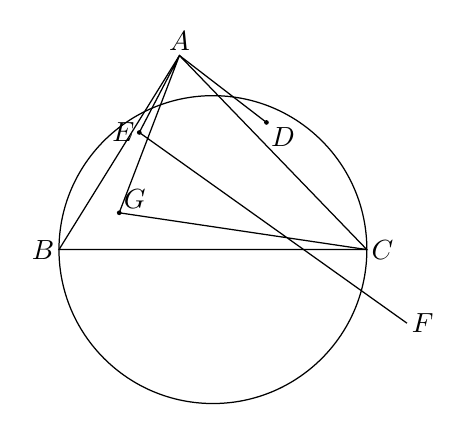
\begin{tikzpicture}[scale=0.85, line width=0.45pt,
  every node/.style={inner sep=1.5pt}]
  \coordinate (B) at (-2.3,0); \coordinate (C) at (2.3,0);
  \coordinate (O) at (0,0); \coordinate (A) at (-0.5,2.9);
  \coordinate (D) at (0.8,1.9); \coordinate (E) at (-1.1,1.75);
  \coordinate (G) at (-1.4,0.55); \coordinate (F) at (2.9,-1.1);
  \draw (O) circle (2.3);
  \draw (A)--(B)--(C)--cycle;
  \draw (A)--(D) (A)--(E)--(F) (A)--(G)--(C);
  \draw (B)--(C);
  \fill (D) circle (0.035) (E) circle (0.035) (G) circle (0.035);
  \node[anchor=south] at (A) {$A$}; \node[anchor=east] at (B) {$B$};
  \node[anchor=west] at (C) {$C$}; \node[anchor=north west] at (D) {$D$};
  \node[anchor=east] at (E) {$E$}; \node[anchor=south west] at (G) {$G$};
  \node[anchor=west] at (F) {$F$};
\end{tikzpicture}
